\documentclass[12pt]{article}
\usepackage[utf8]{inputenc}

%%%%%%%%%%%%
% PACKAGES %
%%%%%%%%%%%%
% Layout
\usepackage{geometry} % Margins
\usepackage{multicol} % Side by side
\usepackage{mwe}      % Minipages

% Network
\usepackage{hyperref} % Links

% Graphics
\usepackage{xcolor}    % Colors
\usepackage{fontspec}  % Custom fonts
\usepackage{graphicx}  % Images
\usepackage{wrapfig}   % Wrapping images
\usepackage{tcolorbox} % Colored box indicators
\usepackage{tikz}      % Progress bars
\usetikzlibrary{positioning} % Relative positioning

%%%%%%%%%%%%%%%%%%%%%
% MACROS & COMMANDS %
%%%%%%%%%%%%%%%%%%%%%
% Vertical separator
\newcommand{\vsep}[1]{
  \vspace{.4cm}
  {\color{#1}\hrule}
  \vspace{.4cm}
}

\newcommand{\skillbar}[3][\textwidth]{
  \def\skilldimen{#3\textwidth}
  \begin{tikzpicture}
    \fill[fill=myGray] (0,0) -- (\textwidth, 0) -- (\textwidth, .2cm) -- (0, .2cm);
    \fill[fill=#2] (0,0) -- (\skilldimen, 0) -- (\skilldimen, .2cm) -- (0, .2cm);
  \end{tikzpicture}
}

\newcommand{\formationstep}[5]{%
  \node [circle, fill=black, minimum size=0.5pt] (circ) at (#1, #2) {\tiny};
  \node [above right=5mm of circ.north east, anchor=north west, text width=0.85\textwidth]{
        \indicator{myAqua}{white}{{\textbf{#3 \textemdash #4}}\\} \parbox{\textwidth}{#5}};
}

%%%%%%%%%
% SETUP %
%%%%%%%%%
% Remove page numbers
\thispagestyle{empty}

% Fonts
\setmainfont{ExploreSans.ttf}

% Geometry
\geometry{a4paper, left=18mm, right=18mm, top=10mm, bottom=15mm}

% Grapghics
\graphicspath{{./Images}}

% Color Shortcuts
\definecolor{myLightGray}{HTML}{f8f8f8}%
\definecolor{myGray}{HTML}{dddddd}%
\definecolor{myAqua}{HTML}{5c9fb3}%
\definecolor{myTurq}{HTML}{4399bc}%
\definecolor{myOrange}{HTML}{ccc365}%
\definecolor{myCyan}{HTML}{42cce3}%
\definecolor{myGreen}{HTML}{1ee296}%
\definecolor{myYellow}{HTML}{ddd959}%
\definecolor{myPink}{HTML}{d43b60}%
%\definecolor{}{HTML}{}%
%\definecolor{}{HTML}{}%

% Colorboxes
\newtcbox{\indicator}[2]{
size=fbox, on line, arc=0pt,boxrule=0pt,
colback=#1,
coltext=#2
}

\newtcbox{\ulbox}[2]{
  standard jigsaw,
  opacityback=0,
  adjust text=Ajg,
  before upper=\strut,
  valign=bottom, box align=base,
  size=fbox, on line, arc=0pt,
  boxrule=0pt, bottomrule=2pt,
  colframe=#1,
  coltext=#2
}

\newtcbox{\sectionbox}[2]{
  standard jigsaw,
  opacityback=0,
  before upper=\strut,
  valign=bottom, box align=base,
  size=fbox, arc=0pt,
  boxrule=0pt, bottomrule=2pt,
  fontupper=\Large,
  halign=left,
  colframe=#1,
  coltext=#2,
}


%%%%%%%%%%%%
% DOCUMENT %
%%%%%%%%%%%%
\begin{document}

%%% Set background color
\pagecolor{myLightGray}

%%% Presentation
\noindent
\begin{tcolorbox}[size=tight, colback=myAqua, boxrule=0pt,
  extrude left by=10cm, extrude right by=10cm]{
    \begin{minipage}{\textwidth}
      \noindent
      \begin{minipage}{3.3cm}
        \noindent
        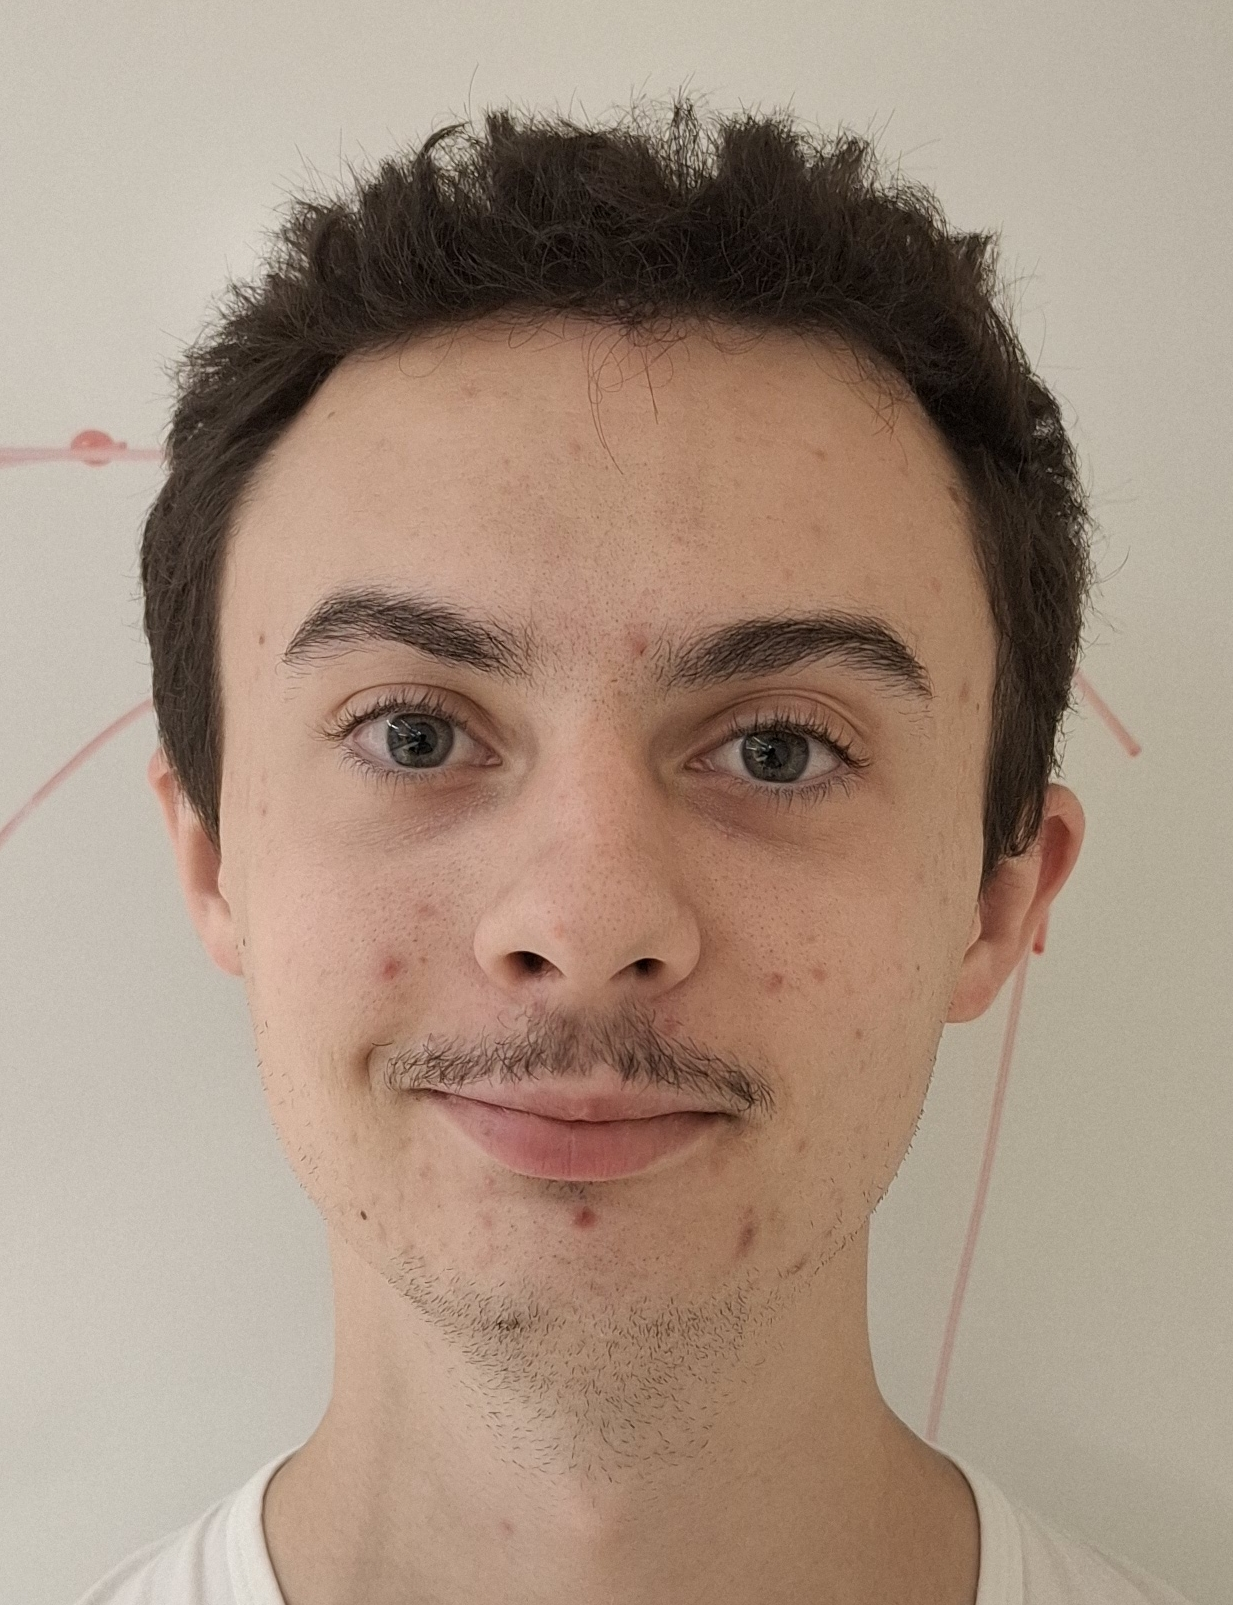
\includegraphics[width=3.3cm]{./Photo.jpg}
      \end{minipage}
      \hfill
      \begin{minipage}{\dimexpr\textwidth - 4cm\relax}
        \color{white}

        {\Huge Bastien Santé}\\
        \vspace{.1cm}
        {\Large Développeur junior de jeux vidéo}

        \vspace{.5cm}
        
        \ulbox{myCyan}{white}{bastien.sante.dev@gmail.com}\  \ulbox{myGreen}{white}{+33 6 26 80 40 87}\par
        
        \ulbox{myOrange}{white}{\href{https://github.com/BastienSANTE}{GitHub}}\ 
        \ulbox{myCyan}{white}{\href{https://www.linkedin.com/in/bastien-sant\%C3\%A9-0bb174320/}{LinkedIn}}\
        \ulbox{myYellow}{white}{\href{https://www.linkedin.com/in/bastien-sant\%C3\%A9-0bb174320/}{Portfolio}}\
        \ulbox{myGreen}{white}{\href{https://www.linkedin.com/in/bastien-sant\%C3\%A9-0bb174320/}{Site personnel}}\
      \end{minipage}
    \end{minipage}
  }
\end{tcolorbox}

\vfill

%%% Description
\noindent\indicator{myTurq}{white}{\textbf{PROFIL}} Je suis un jeune développeur, passionné par les RPG et intéressé par l'architecture logicielle, qui a à c{\oe}ur d'implémenter des systèmes efficaces, simples d'emploi et flexibles pour les jeux vidéo. J'ai un intéret particulier pour les interfaces utilisateur et la typographie, que je pratique en tant qu'amateur.\\\\
\noindent\indicator{myGreen}{white}{\textbf{PASSIONS}} Course à pied, Dessin digital, Modélisation 3D, Mise en page \LaTeX\par

%\vsep{myGray}

\vfill

%%% Skills
\noindent%
\begin{minipage}[t]{0.45\linewidth}
  \begin{minipage}[t]{\textwidth}
    %\renewcommand{\baselinestretch}
    \sectionbox{myAqua}{black}{\makebox[\textwidth][l]{Compétences}}
    Développement en C\#\\
    \skillbar{myYellow}{0.8}

    Développement en C++ \& Blueprints\\
    \skillbar{myOrange}{0.7}
    
    Design UI/UX (UMG, UI Toolkit)\\
    \skillbar{myGreen}{.8}
    
    Gestion de projet avec Git et Perforce\\
    \skillbar{myAqua}{0.7}

    Gestion de systèmes Linux (Debian)\\
    \skillbar{gray}{.8}\\

    \textbf{Ouverture d'esprit} \textemdash\ J'accepte facilement le changement et la nouveauté dans l'organisation\\

    \textbf{Analyse} \textemdash\ Je préfère prendre plusieurs approches à un problème\\

    \textbf{Apprentissage} \textemdash\ J'aime me former également en dehors du travail, tout en assurant une veille technique\\
  \end{minipage}
  
  \begin{minipage}[t]{\textwidth}
    \sectionbox{myAqua}{black}{\makebox[\textwidth][l]{Participations}}
    God's Vault \textemdash\ Survival horror sur Unreal Engine 5, projet de 4\textsuperscript{ème} année\\
    Terminus 6 \textemdash\ Jeu de réflexion "escape game" VR sous Unity 6\\
    Clawster \textemdash\ Jeu mobile sous Unity 6
  \end{minipage}
\end{minipage}
%
%---------------------------%
\hfill % Space between sides
%---------------------------%
%
\begin{minipage}[t]{0.45\linewidth} % Nested minipages for vertical alignment

  % Learningx
  \begin{minipage}[t]{\textwidth}
    \sectionbox{myAqua}{black}{\makebox[\textwidth][l]{Formation}}
    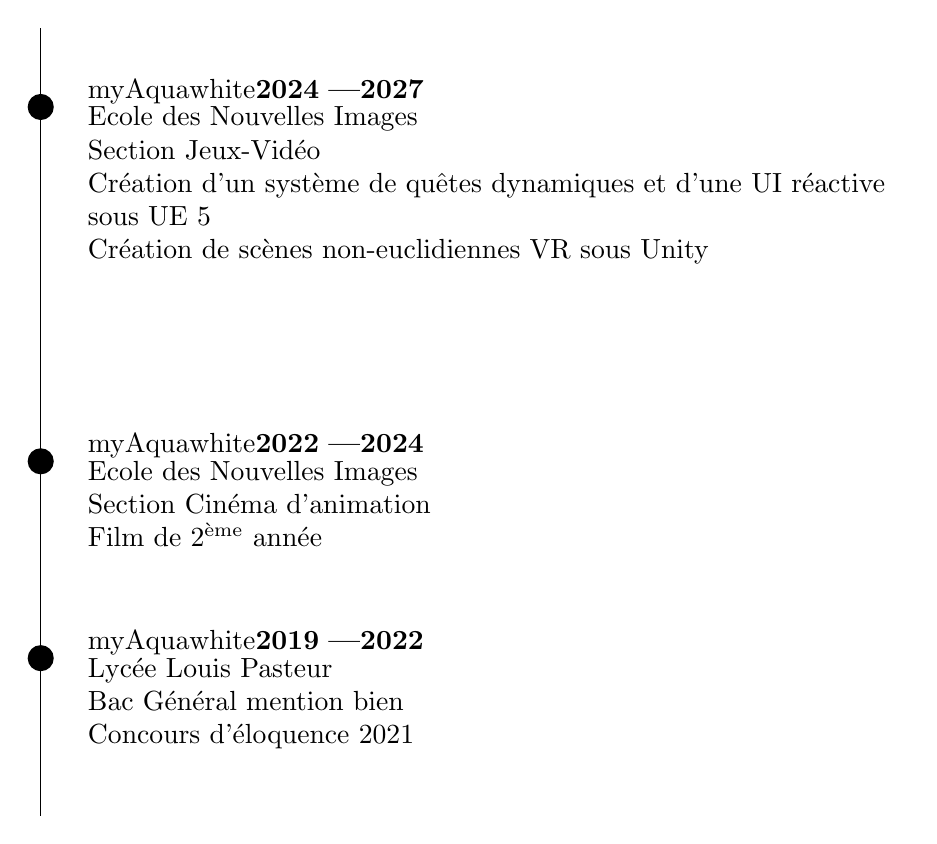
\begin{tikzpicture}
      \draw (0,0) -- (0, -10);

      % ENSI Game
      \formationstep{0}{-1}{2024}{2027}{
        Ecole des Nouvelles Images\\Section Jeux-Vidéo\\
        Création d'un système de quêtes dynamiques et d'une UI réactive sous UE 5\\
        Création de scènes non-euclidiennes VR sous Unity\\
      }

      % ENSI Anim
      \formationstep{0}{-5.5}{2022}{2024}{Ecole des Nouvelles Images\\Section Cinéma d'animation\\
      Film de 2\textsuperscript{ème} année};

      % HS
      \formationstep{0}{-8}{2019}{2022}{Lycée Louis Pasteur\\Bac Général mention bien\\Concours d'éloquence 2021};
    \end{tikzpicture}
  \end{minipage}

  
  \vsep{myLightGray}
  
  % Languages
  \begin{minipage}[t]{\textwidth}
    \sectionbox{myAqua}{black}{\makebox[\textwidth][l]{Langues}}
    Anglais \hfill \indicator{myCyan}{white}{C2}\\
    \skillbar{myCyan}{0.97}
    Italien \hfill \indicator{myGreen}{white}{B1}\\
    \skillbar{myGreen}{0.68}
    Japonais \hfill \indicator{myPink}{white}{Débutant}\\
    \skillbar{myPink}{0.1}
  \end{minipage}
\end{minipage}

% Credits
\vfill
\hfill \footnotesize{CV réalisé en \LaTeX\ avec Emacs\ \ulbox{myOrange}{black}{\href{https://github.com/BastienSANTE/CV/blob/main/CV/CV.tex}{\footnotesize sans IA générative}}}

\end{document}
